\documentclass[tikz,border=2pt]{standalone}
\usepackage{amsmath}
\usepackage{pgfplots}
\pgfplotsset{compat=1.18}
\usetikzlibrary{arrows.meta}
\begin{document}
% Service time 1.5: an always-busy server completes U(t) jobs (steps at 1.5k, rate mu = 2/3);
% with arrivals at 1,4,5,8,9,12 the actual departures D(t) step at 2.5,5.5,7,9.5,11 (rate delta = 1/2).
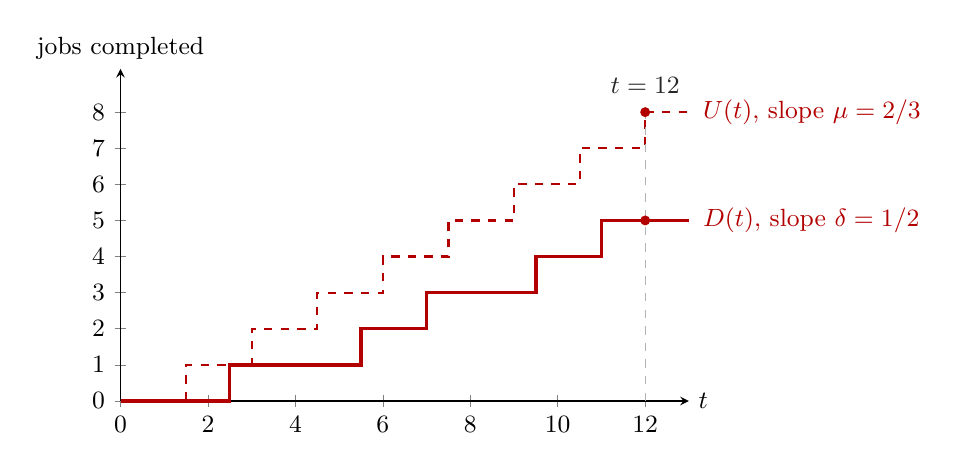
\begin{tikzpicture}[font=\small, >={Latex[length=2mm]}]
  \begin{axis}[
    axis lines=left, xmin=0, xmax=13, ymin=0, ymax=9.2,
    xtick={0,2,4,6,8,10,12}, ytick={0,1,...,8},
    xlabel={$t$}, ylabel={jobs completed},
    xlabel style={at={(axis description cs:1,0)}, anchor=west},
    ylabel style={rotate=-90, at={(axis description cs:0,1)}, anchor=south},
    width=8.8cm, height=5.8cm, clip=false
    ]
    \addplot[red!70!black, thick, dashed, const plot]
      coordinates {(0,0) (1.5,1) (3,2) (4.5,3) (6,4) (7.5,5) (9,6) (10.5,7) (12,8) (13,8)};
    \addplot[red!70!black, very thick, const plot]
      coordinates {(0,0) (2.5,1) (5.5,2) (7,3) (9.5,4) (11,5) (13,5)};
    \draw[gray!60, thin, dashed] (axis cs:12,0) -- (axis cs:12,8);
    \node[red!70!black, anchor=west] at (axis cs:13.1,8) {$U(t)$, slope $\mu=2/3$};
    \node[red!70!black, anchor=west] at (axis cs:13.1,5) {$D(t)$, slope $\delta=1/2$};
    \fill[red!70!black] (axis cs:12,8) circle (1.8pt);
    \fill[red!70!black] (axis cs:12,5) circle (1.8pt);
    \node[gray!30!black, anchor=south] at (axis cs:12,8.25) {$t=12$};
  \end{axis}
\end{tikzpicture}
\end{document}
